

\noindent 
\textbf{\stepcounter{zadatak}
\thecjelina.\thezadatak.}
Vanjska sila iznosa $\vec{F_0}=18\ N$ djeluje pod kutom od $\alpha=28 ^\circ$ prema horizontali na blok mase $m=3\ kg$. Izračunajte iznos 
ubrzanja kada je kinetičko trenje između bloka i podloge $\mu_k=0,4$.


\begin{figure}[h]%{r}{0.4\textwidth} % Inline image example
  \begin{center}
    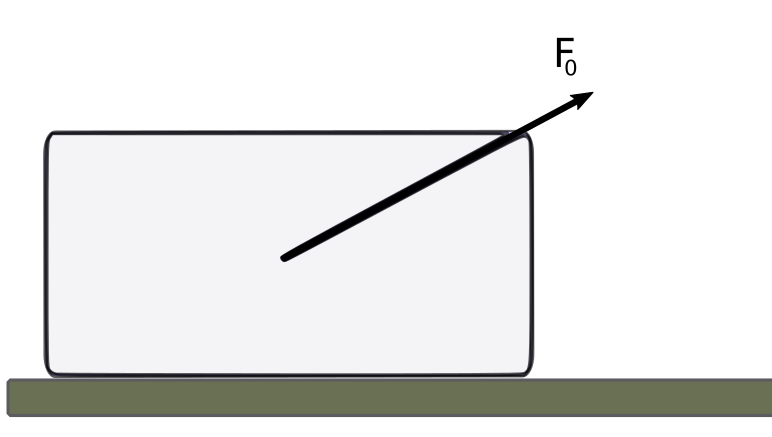
\includegraphics[scale=0.29]{03_Dinamika_materijalne_tocke/blok_Zadatak_4_1.png}
  \end{center}
  %\caption{Fish}
\end{figure}
